\chapter{Entwurf}
\label{sec:entwurf}


\section{Raspberry Pi}
Zur Überführung des Systems in die Realität benutze ich Raspberry Pi Version B als Schnittstelle zwischen Computermodell und der Umsetzung auf Hardware samt Aktuatoren (Motoren, Regler usw.). Dieser gibt die Steuersignale direkt an die Aktuatoren weiter, die letztlich die Geschwindigkeit und Lenkung bestimmen. 
Raspberry Pi ist ein kostengünstiger Einplatinen-Computer, der in etwa die Größe einer Kreditkarte hat und auf dem Linux-Betriebssysteme laufen. Raspberry Pi basiert auf ARM® Cortex® A-Prozessoren und hat verschiedene Ausgänge für Verbindungen mit Peripheriegeräten wie Stereo-Audio, digitales Video, USB und Ethernet.


\section{Realisierung auf dem RaspberryPi}
\label{sec:Umsetzung}
Bei Matlab/Simulink können Modelle mit Hilfe der richtigen Support Packages direkt auf der Hardware (den Raspberry Pi 2 Version B) ausgeführt werden. Dabei unterscheiden sich Matlab und Simulink wie folgt: \\
Mittels Ethernetkabel werden bei der Ausführung von Modellen in Matlab Daten von der Hardware eingelesen oder Informationen zur Hardware gesendet.
Anders als bei Matlab wird bei Simulink der Algorithmus direkt auf der Hardware ausgeführt.
Dazu generiert das Simulink Support Package beim Ausführen des Modells Code, der anschließend auf dem Raspberry Pi ausgeführt wird.
Mit dem Simulink Support Package für Raspberry Pi lassen sich Algorithmen entwickeln, die eigenständig auf dem Raspberry Pi ausgeführt werden können. Das Support Package erweitert Simulink um Blöcke, mit denen sich die digitale Pins des Raspberry Pi steuern lassen, sowie Daten eingelesen und geschrieben werden können. Hat man erst ein funktionierendes Simulink-Modell erstellt, lässt sich der dazugehörige Algorithmus auf den Raspberry Pi herunterladen und dort eigenständig ausführen. \\
Mittels Support Package kann über eine Remote Verbindung mit dem Raspberry Pi kommuniziert werden. Dieser steuert Peripheriegeräte und kann Daten von Sensoren einlesen. MATLAB arbeitet auf dem Raspberry Pi nicht als Standalone, denn der MATLAB-Code wird nicht lokal auf der Hardware ausgeführt. \\
Die General-Purpose-Input-Outputs (GPIO) können nur boolsche Werte annehmen. Sie dienen ausschließlich der logischen Signalweitergabe und nicht als Strom oder Spannungsquelle. \\
Servomotoren können mit einem einzigen GPIO gesteuert werden. Die Rotation und der damit resultierende Lenkwinkel entstehen durch die Dauer des Impulses am Pin. Der Winkel hängt dabei vom spezifischen Servo ab. \\
\\

Die GPIO bilden die Schnittstelle zwischen dem Raspberry Pi und digitalen Schaltungen. Nachdem man über die Konsole in MATLAB Verbindung zu der Hardware aufgebaut hat, lässt sich via PuTTY eine Konsole öffnen, in der man interaktive Befehle auf dem Raspberry Pi ausführen lassen kann:
\lstset{language=bash}          
\begin{lstlisting}[frame=single]
rpi = raspi();
openShell(rpi)
\end{lstlisting}
Nach dem Einloggen auf der Hardware, lassen sich die einzelnen GPIO austeuern. Diese befinden sich als Dateien im Verzeichnis /sys/class/gpio. Um einen Pin ansteuern zu können, muss man ihn vorher 'exportieren'. Im folgendem Beispiel wird das an Pin 17 demonstriert:
\lstset{language=bash}          
\begin{lstlisting}[frame=single]
echo "17" > /sys/class/gpio/export
\end{lstlisting}
Dadurch wird ein neuer Ordner innerhalb von /sys/class/gpio/gpio17/ erstellt, mit dem nun gearbeitet werden kann. Das geschieht, indem man den Pin als Input oder als Output definiert, also ob man Signale lesen oder schreiben möchte: 
\lstset{language=bash}          
\begin{lstlisting}[frame=single]
echo "out" > /sys/class/gpio/gpio17/direction
\end{lstlisting}
Der GPIO ist binär. Er kann entweder eine Spannung von 3,3 Volt haben, oder keine. Er kann lediglich diese beiden Zustände annehmen und lässt sich nun ansteuern:
\lstset{language=bash}          
\begin{lstlisting}[frame=single]
echo "1" > /sys/class/gpio/gpio17/value
\end{lstlisting} 

Alternativ lassen sich die GPIO auch über WiringPi steuern. WiringPi ist ein Framework, das die Einbindung in Programmiersprachen wie Python oder C ermöglicht.  
Darüber hinaus kann es mit den mitgelieferten Bibliotheken in C, C++, Python, Java und php eingebunden werden. Es benutzt eine andere GPIO-Belegung, aber durch die Option -g wird die normale Raspberry Pi Belegung genutzt. Es lassen sich die gleichen Befehle ausführen, aber mit anderem Syntax:
\lstset{language=bash}          
\begin{lstlisting}[frame=single]
gpio export 17 out 
gpio -g write 17 1 
\end{lstlisting}
Der eigentliche Vorteil liegt aber darin, dass eine Bibliothek von Befehlssätzen, die mit WiringPi installiert werden, in C-Code integriert werden kann, wodurch sich mit der Programmiersprache direkt die Pins ansteuern lassen. Weil auch unser Modell aus Simulink in C-Code kompiliert wird, besteht hier die Möglichkeit, diese beiden losen Fäden zu verbinden. \\
Bei jedem Simulink Modell, das erfolgreich auf dem Raspberry Pi läuft, wird eine ELF (Executable and Linking Format) erstellt. \\ \\

Testweise wurde ein MOSFET an den GPIO 17 angeschlossen. Dieser dient als Schalter: Liegt eine Spannung am richtigen der drei Eingänge des MOSFETs an, so schließt sich der Schalter zwischen den zwei anderen Eingängen und Strom kann fließen. An dem MOSFET waren noch eine LED sowie eine Stromquelle angeschlossen. Solange an dem Pin eine logische 0 anlag, passierte nichts, aber durch die Veränderung des Wertes, schloss der MOSFET den Stromkries und das LED leuchtete (vgl. Abbildung 5.1). \\
\begin{figure}[htb]
  \centering  
  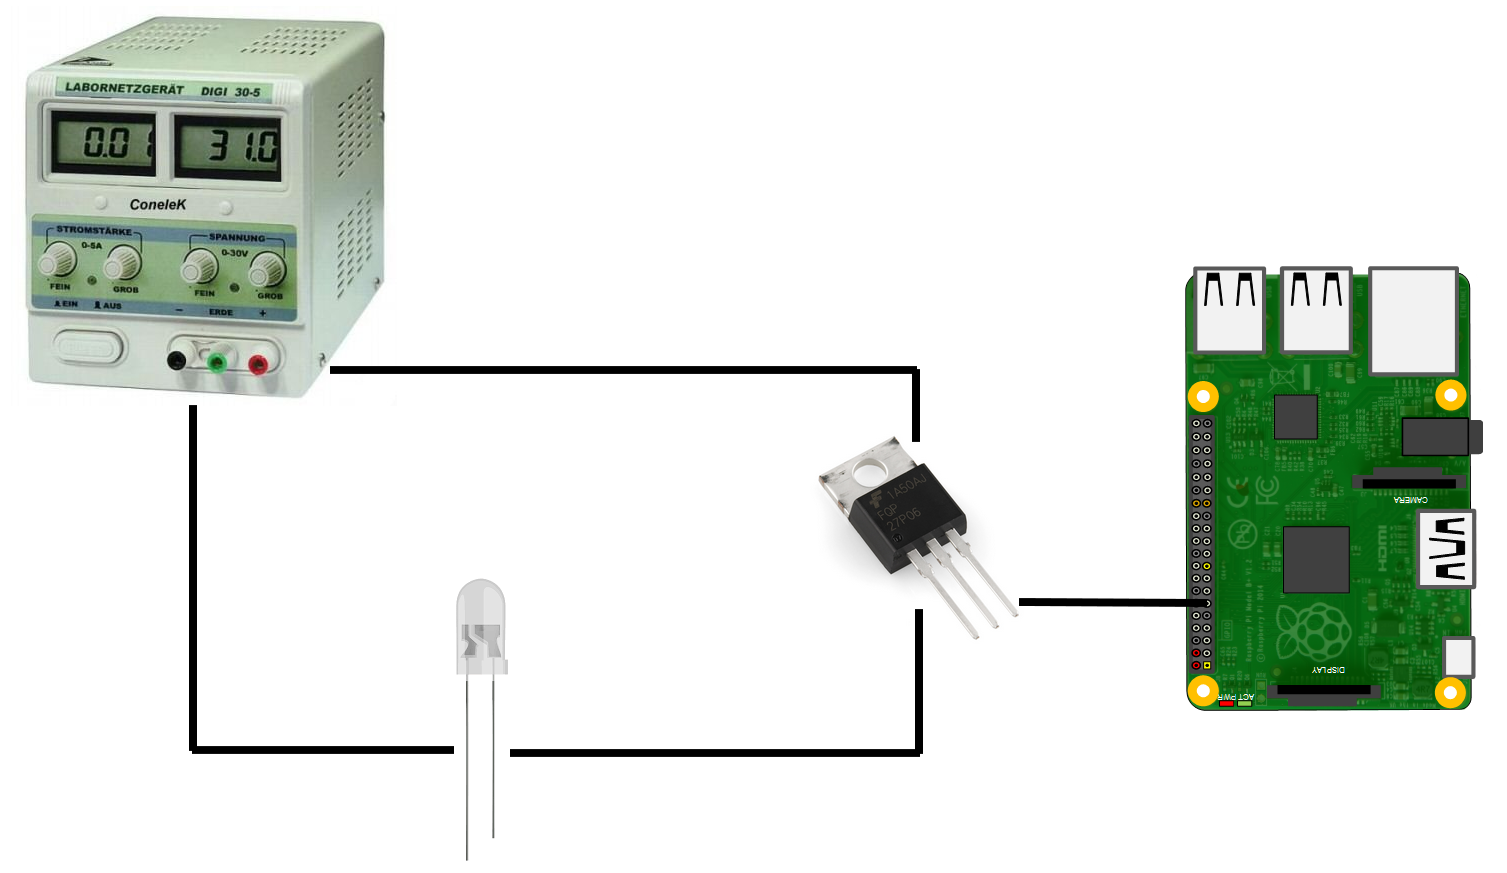
\includegraphics[scale=1]{img/versuchsaufbau.png}
  \caption{Versuchsaufbau der Ansteuerung des GPIO 17}
  \label{fig:starwars}
\end{figure}


Die nächste Überlegung war, wie man überhaupt anhand von Signalen Motoren steuern kann. Zur Lenkung empfiehlt sich ein Servo-Motor, der im Gegensatz zu Schrittmotoren bereits mit einem Pin auskommt und über die Länge des Impulses den Lenkwinkel bestimmen kann, allerdings wird in unserem gewähltem Fahrzeugmodell die Lenkung über die unterschiedlichen Geschwindigkeiten beider Räder bestimmt, also braucht man einen Schrittmotor. Am besten werden Motoren über PWM (Pulsweitenmodulation) geregelt, womit wiederholte Signale in regelmäßigen Abständen übertragen werden. Das kann man sich so vorstellen: Das Signal, also die Spannung am GPIO, wird getaktet. In gleichmäßigen Abständen wechselt es zwischen 1 und 0, zwischen an und aus, also ob 3,3 Volt anliegen oder nicht. Dadurch lässt sich die durchschnittliche Spannung regulieren. Ist der Impuls/Pulsweite kurz, gibt es einen Längeren Zeitraum, in dem keine Spannung anliegt, und der Motor sollte langsamer werden. Um das veranschaulich zu verifizieren wurde ein weiteres Simulink Modell gebaut (siehe Abbildung 5.2). \\
\begin{figure}[htb]
  \centering  
  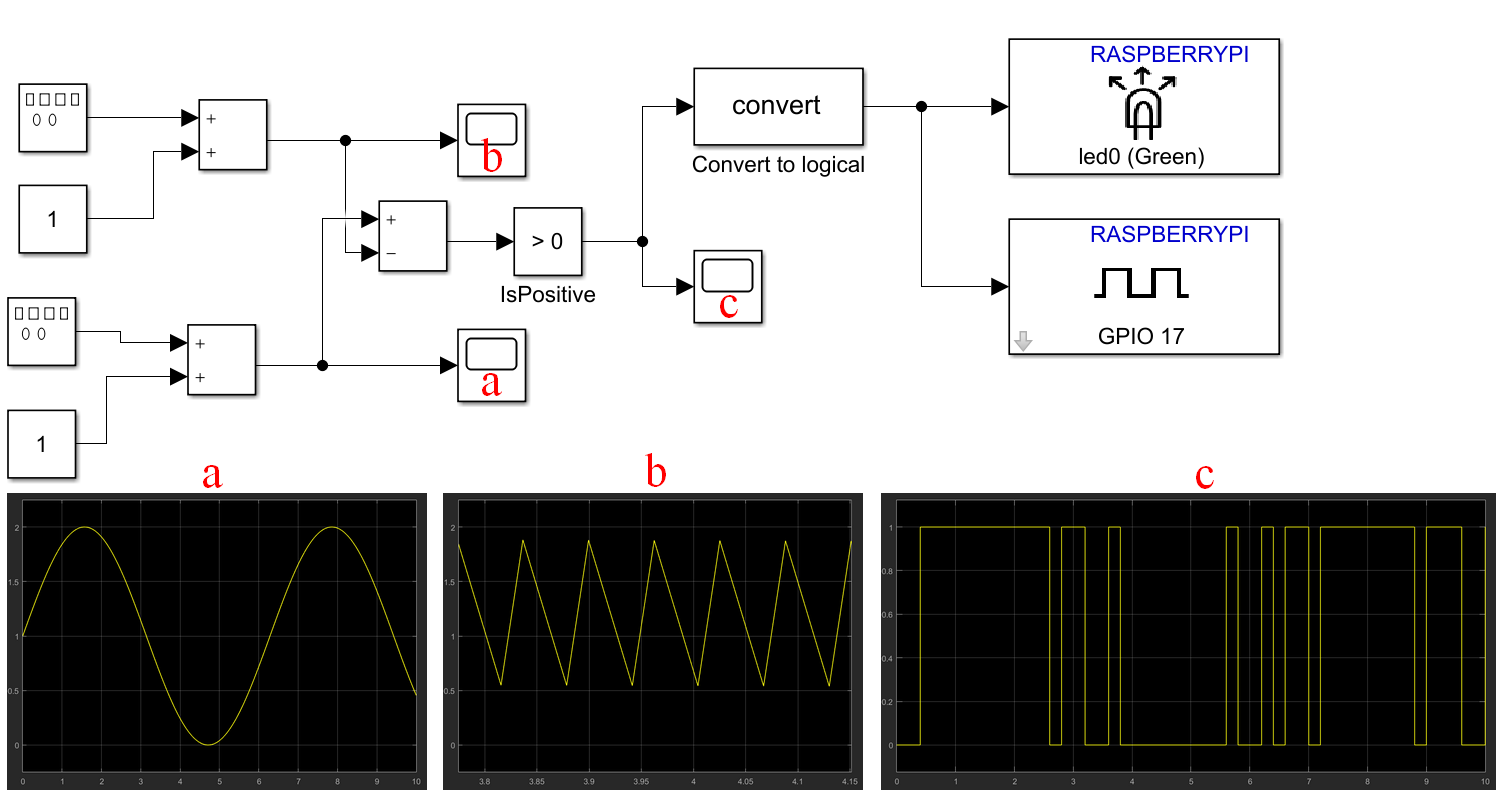
\includegraphics[scale=1]{img/saw.png}
  \caption{Sinusförmig verändernde Helligkeit}
  \label{fig:Sägezahnmodell zum Kreisförmigen Dimmungsverlauf einer LED}
\end{figure}
Dem Modell dienen zwei Impulsgebern als Input. Der untere in der Form einer Sinuskurve und der obere als Sägezähne. Anhand der Sägezähne lässt sich das Signal gut regulieren. Die Höhe der oberen Spitzen des Sägezahns ist dabei der maximale Impuls, der (in diesem Fall an LED und GPIO17) weitergegeben werden kann. Ziel dieses Beispieles ist es, anhand der Sinuskurve, das Signal jeweils so zu regulieren, dass das LED am hellsten ist, wenn die Sinuskurve einen Hochpunkt hat, das LED aus ist, bei einem niedrigen Maximalpunkt und dass das LED dazwischen jeweils so gedimmt ist, wie die aktuelle Position auf der Sinuskurve im Verhältnis zur Amplitude steht. Auf diese Weise lassen sich analoge Geräte wie Motoren von digitalen Schaltungen (die der Raspberry Pi wie alle anderen Microcontroller auch ausgibt) ansteuern. Abbildung 5.3 dient als Erklärungshilfe:
\begin{figure}[htb]
  \centering  
  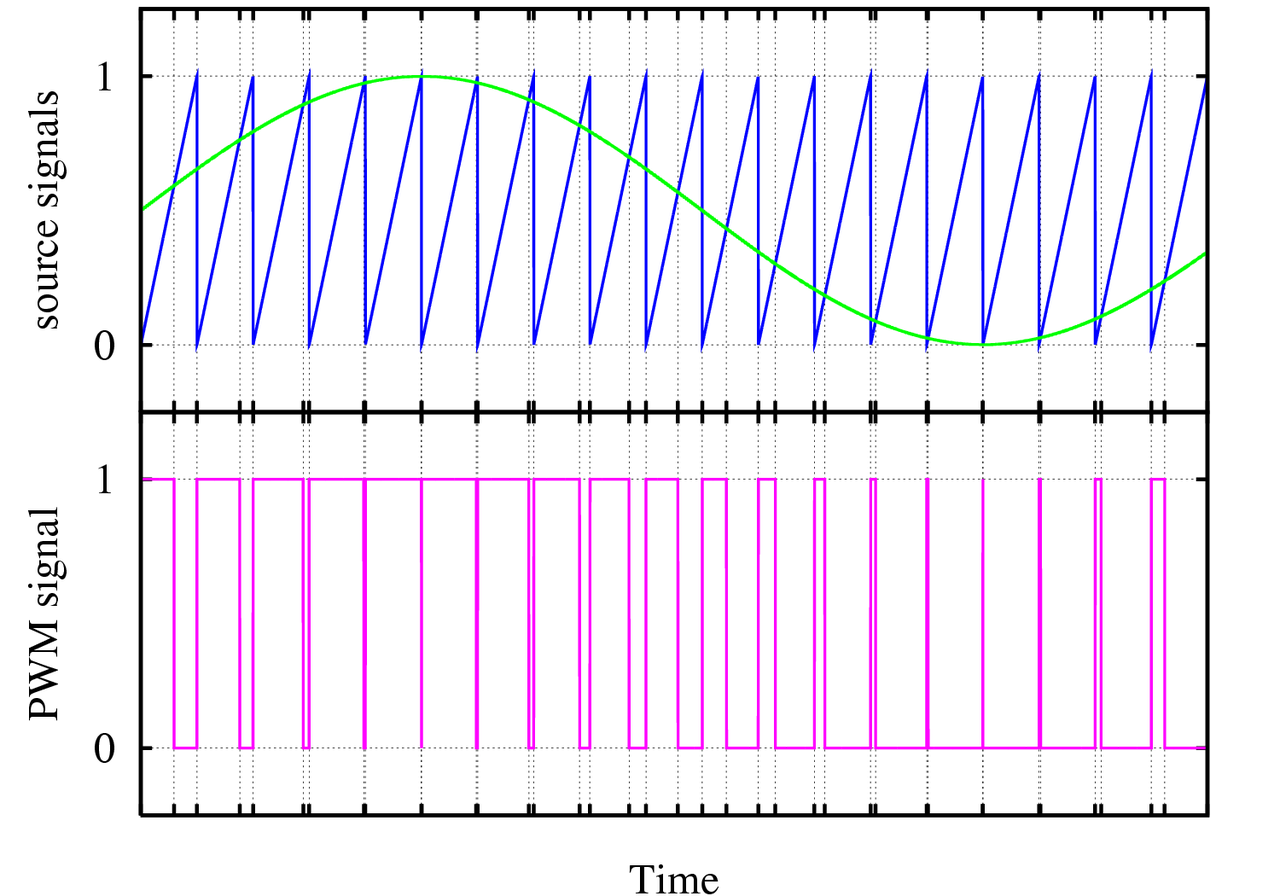
\includegraphics[scale=0.3]{img/sinussaw.png}
  \caption{Bei der Überlagerung von Sinuskurve und Sägezahnförmigem Signal, kann erstere durch die Schnittpunkte in ein analoges PWM-Signal umwandeln \\ Quelle: Wikipedia, \url{https://de.wikipedia.org/wiki/Pulsweitenmodulation}, stand 12.6.2018}
  \label{fig:Pulsweitenmodulation}
\end{figure}
Bei der Ausführung dieses Modells, ändert sich die Helligkeit der LED sinusartig. Das bedeutet dass die Pulsweitenmodulation funktioniert. Genau wie beim Test der LEDs, kann dieses Prinzip auch für einen Motor in Einsatz kommen, um dessen Drehmoment zu regulieren. So lässt sich jetzt nicht nur eine Sinuskurve umsetzten, sondern eben auch die gewünschten Geschwindigkeitsänderungen unseres Simulink-Modells. Statt der Sinuskurve als Eingang braucht man für die Realisierung der Geschwindigkeitsregelung am Raspberry Pi nur die aktuell gewünschte Soll-Geschwindigkeit anzugeben. Dies allerdings als Wert zwischen 0 und 1.  \\ \\

In diesem Kapitel wurde die Verbindung zwischen Modell und Hardware des Raspberry Pi erstellt und getestet. Genauer, es wurden die GPIOs des Raspberry Pi angesteuert, und überlegt, wie sich damit Motoren regeln lassen. Das zufriedenstellende Ergebnis war, dass sich mittels PWM die Aktuatoren (über die GPIOs) so regeln lassen, wie es für das Fahren eines Autos notwendig ist.


